%=================SAMPLE FIGURE================


% --------Float Placement Options-------------
% ht → Prefer here, otherwise top of page.
% hb → Prefer here, otherwise bottom of page.
% htb → Try here, then top, then bottom.
% htbp → The most common (default): try here, top, bottom, or on a dedicated float page.
% h → here: Place the float approximately at the same location in the source text.
% t → top: Place the float at the top of a page.
% b → bottom: Place the float at the bottom of a page.
% p → page of floats: Place the float on a dedicated page that contains only floats (figures/tables).
% H → Absolutely HERE, no floating allowed. The figure is placed exactly at the point in the source code.


\begin{figure}[!ht]
    \centering
    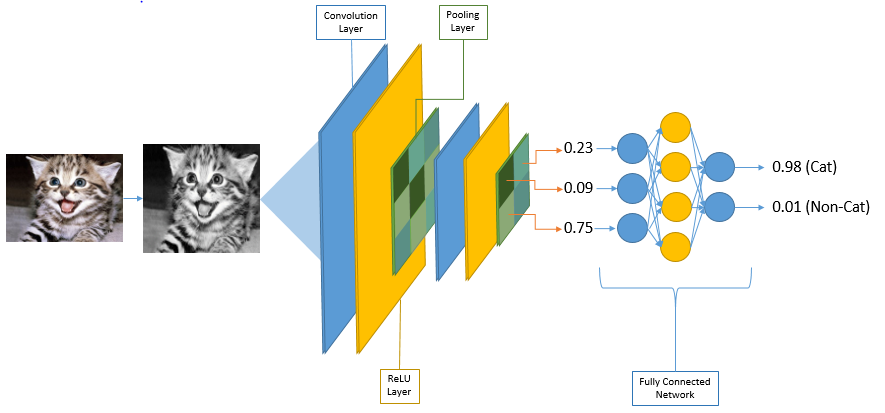
\includegraphics[width=3in]{figure/Image Classification Using Neural Networks.png}
    \caption{Figure description}
    \label{label_name}
\end{figure}


\begin{figure}[!ht]
    \centering
    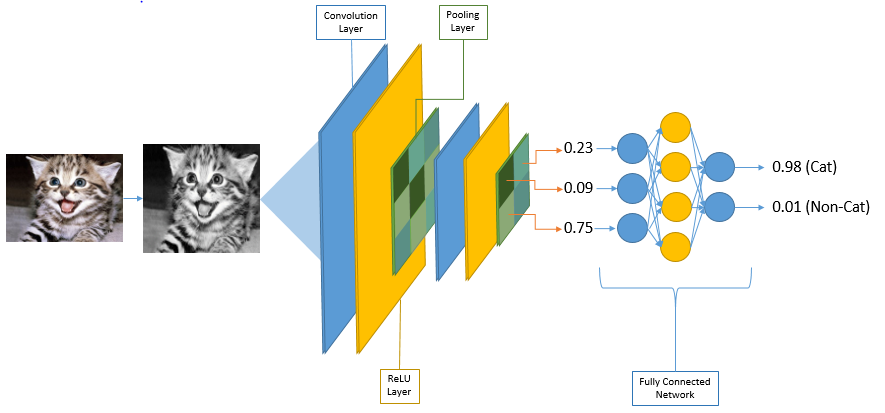
\includegraphics[width=3in]{figure/Image Classification Using Neural Networks.png}
    \caption{Figure description}
    \label{label_name}
\end{figure}


\begin{figure}[H]
    \centering
    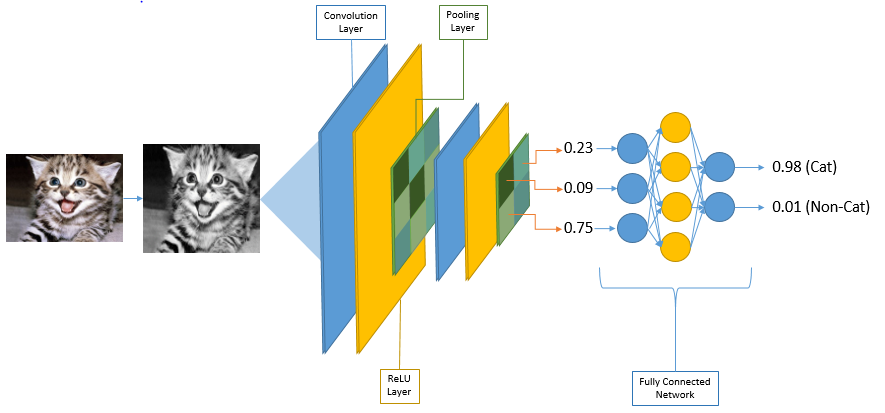
\includegraphics[width=3in]{figure/Image Classification Using Neural Networks.png}
    \caption{Figure description}
    \label{label_name}
\end{figure}




%=================SAMPLE TABLE================

% \begin{table}[!ht]
% \begin{table}[H]

% EXAMPLE 1:

\begin{table}[H]
    \centering
        \begin{tabular}{|l|c|c|}
        \hline
            \thead{Column 1} & \thead{Column 2} & \thead{Column 3}  \\ \hline
            Value 1 & Value 2 & Value 3     \\ \hline
            Value 4 & Value 5 & Value 6     \\ \hline
            Value 7 & Value 8 & Value 9     \\ \hline            
        \end{tabular}
    \caption{This is table description}
    \label{tab:reference}
\end{table}


% EXAMPLE 2:

\begin{table}[H]
    \centering
        %use cm--> for centimeter, in--> for inch, pt--> for points
        \begin{tabular}{|c|p{5cm}|p{8cm}|}
        \hline
            \thead{Column 1} & \thead{Column 2} & \thead{Column 3}  \\ \hline
            Value 1 & Value 2 & Value 3     \\ \hline
            Value 4 & Value 5 & Value 6     \\ \hline
            Value 7 & Value 8 & Value 9     \\ \hline            
        \end{tabular}
    \caption{This is table description}
    \label{tab:reference}
\end{table}


% EXAMPLE 3:

\begin{table}[H]
    \centering
        %use cm--> for centimeter, in--> for inch, pt--> for points
        \begin{tabular}{|c|m{5cm}|m{8cm}|} 
        \hline
            \thead{Column 1} & \thead{Column 2} & \thead{Column 3}  \\ \hline
            Value 1 & Value 2 & Value 3     \\ \hline
            Value 4 & Value 5 & Value 6     \\ \hline
            Value 7 & Value 8 & Value 9     \\ \hline            
        \end{tabular}
    \caption{This is table description}
    \label{tab:reference1}
\end{table}

% If you want to keep table width within page width then use following syntax. Change number of columns according to requirement.


% EXAMPLE 4:

\begin{table}[H]
% To make table description justified use this captionsetup
% \captionsetup{justification=justified,singlelinecheck=false}
\caption{Table Description} 
\label{label_name}

\centering
\resizebox{\textwidth}{!}{ 
\begin{tabular}{|c|c|c|c|c|c|c|}
\hline

\thead{Column 1} & \thead{Column 2} & \thead{Column 3} & \thead{Column 4} & \thead{Column 5} & \thead{Column 6} & \thead{Column 7} \\ \hline

&   &   &   &   &   & \\ \hline

&   &   &   &   &   & \\ \hline

&   &   &   &   &   & \\ \hline

\end{tabular}}
\end{table}




%=================SAMPLE EQUATION================

\begin{equation}
s=ut+\frac{1}{2}ft^2
\end{equation}


\[
  f(x) =
  \begin{cases}
    x^2, & x \ge 0, \\
    -x,  & x < 0.
  \end{cases}
\]


If you want a label then use following syntax:

\begin{equation}
  f(x)=
  \begin{cases}
    x^2 & x\ge0,\\
    -x  & x<0.
  \end{cases}
\end{equation}


Use following syntax for multiline equation

\begin{align}
  F(x) &= \int_0^x \left( a t^2 + b t + c \right) dt \nonumber\\
       &= \left[\tfrac{a}{3}t^3 + \tfrac{b}{2}t^2 + ct\right]_{0}^{x} \\
       &= \tfrac{a}{3}x^3 + \tfrac{b}{2}x^2 + c x. \nonumber
\end{align}



%=============== Celling, Floor, Log===========

$2^{(m-p)} \times 2^p=2^m$


$\left \lceil{x}\right \rceil $




  \begin{equation*}
    \floor*{\frac{x}{2}} \leq \frac{x}{2} \leq \ceil*{\frac{x}{2}}
  \end{equation*}




    $A(n) \in \Theta(n^{\log_b a}) = \Theta(n^{\log_2 2} ) = \Theta(n)$


$\left \lceil{log_2 M}\right \rceil =m$
\\\\
$\left \lceil{log_2 L}\right \rceil =l$
\\\\
$\left \lceil{log_2 P}\right \rceil =p$



    The 2D Gaussian function is given by:

\[
\mathlarger{G(x, y) = \frac{1}{2\pi\sigma^2} e^{-\frac{(x^2 + y^2 )}{2\sigma^2}}}
\]

where:
\begin{itemize}
    \item \(G(x, y)\) is the value of the Gaussian function at the point \((x, y)\),
    \item \(\sigma\) is the standard deviation of the Gaussian distribution,
    \item \(\exp\) denotes the exponential function.
\end{itemize}





% ========================Common Symbols \& Operators================

% Binary ops and relations
$a \pm b, \times, \div, \cdot, a \approx b, a \le b, a \ge b$

% Set symbols
$\in, \notin, \subseteq, \cup, \cap, \emptyset$

% Logic
$\land, \lor, \lnot, \Rightarrow, \Leftrightarrow$

% Other
$\infty, \partial, \nabla, \forall, \exists$





% ============Fractions, Roots, Summation, Integrals================

% Fractions
$\frac{a+b}{c+d}$

% Roots
$\sqrt{x}$

$\sqrt[n]{x+1}$


% Sums and products
\[
  \sum_{i=1}^n i^2, \qquad \prod_{k=1}^m k
\]

% Integrals
\[
  \int_0^1 x^2 \, dx, \qquad \iint_{D} f(x,y)\, dA, \qquad \oint_C \vec{F}\cdot d\vec{r}
\]


% Limit
\[
  \lim_{x\to 0}\frac{\sin x}{x} = 1
\]







%=================SAMPLE MATRIX================

% EXAMPLE 1:

\[
X = 
    \begin{bmatrix}
    10 & 20 & 30 \\
    40 & 50 & 60 \\
    70 & 80 & 90
    \end{bmatrix}
\] 
    
% EXAMPLE 2:    
\[
Let ~Y = 
\begin{bmatrix}
-1 & 0 & 1 \\
-1 & 0 & 1 \\
-1 & 0 & 1
\end{bmatrix}
\] 

% EXAMPLE 3:

\[
Let ~X = 
    \begin{bmatrix}
    -1 & 0 & 1 \\
    -1 & 0 & 1 \\
    -1 & 0 & 1
    \end{bmatrix}
\] 

\[
and ~Y = 
    \begin{bmatrix}
    -1 & -1 & -1 \\
    0 & 0 & 0 \\
    1 & 1 & 1
    \end{bmatrix}
\]

% EXAMPLE 4:

Let’s assume that an image matrix is given as: 
     \[
    \left[ {\begin{array}{cccc}
    3 & 6 & 6 & 8\\
    5 & 3 & 1 & 4\\
    8 & 6 & 5 & 1\\
    4 & 8 & 2 & 3\\
    \end{array} } \right]
    \]

% EXAMPLE 5:
     \[
    \left[ {\begin{array}{ccc}
    CB_R & CB_G & CB_B \\
    r_1 & g_1 & b_1 \\
    r_2 & g_2 & b_2 \\
    r_3 & g_3 & b_3 \\
    :&:&\\
    r_n&g_n&b_n \\
    \end{array} } \right]
    \]


% EXAMPLE 6:

     \[
    \left[ {\begin{array}{ccc}
    CB_Y & CB_{Cb} & CB_{Cr} \\
    y_1 & Cb_1 & Cr_1 \\
    y_2 & Cb_2 & Cr_2 \\
    y_3 & Cb_3 & Cr_3 \\
    :&:&\\
    y_n&Cb_n&Cr_n \\
    \end{array} } \right]
    \]

%=================SAMPLE ALGORITHM================

        \begin{algorithm}[!ht]
        \RaggedRight
        \caption{Name of the Algorithm}
        \label{label_name}
        \algorithmicrequire \quad Input description \\
        \algorithmicensure \quad Output description.
        
        \begin{algorithmic}[1]
            \State Statement 1
            \State Statement 2
            \State Statement 3  
                \For{$i \gets 1$ to m} \qquad \qquad /*m=write what m indicates*/
                    \For{$j \gets 1$ to n} \qquad /*n= write what n indicates*/
                    \State Statement 4
                    \State Statement 5
                    \State Statement 6 
                \EndFor
            \EndFor
            \State Statement 7 
            \State Statement 8 
            
    \end{algorithmic}
    \end{algorithm}


%=============SAMPLE LISTING=====================

% -----Ordered List or Numbered List----------

% \begin{enumerate}
% \begin{enumerate}[label=(\arabic*).]
% \begin{enumerate}[label=\textbf{(\arabic*).}]
% \begin{enumerate}[label=\alph*.]
% \begin{enumerate}[label=(\alph*).]
% \begin{enumerate}[label=\textbf{(\alph*).}]
%     \item Point 1
%     \item Point 2
%     \item Point 3
%     \item Point 4
%     \item Point 5
% \end{enumerate}


\begin{enumerate}
    \item Point 1
    \item Point 2
    \item Point 3
    \item Point 4
    \item Point 5
\end{enumerate}



\begin{enumerate}[label=(\arabic*).]
    \item Point 1
    \item Point 2
    \item Point 3
    \item Point 4
    \item Point 5
\end{enumerate}



%-----Nested List--------------
\begin{enumerate}
    \item Point 1
    \item Point 2
    \item Point 3
    \item Point 4
    \item Point 5
    \begin{enumerate}
        \item Point 6
        \item Point 7
        \item Point 8
    \end{enumerate}
\end{enumerate}



%-------Unordered List or Bulleted List-----------

% List Style-1
\begin{itemize}
    \item Point 1
    \item Point 2
    \item Point 3
    \item Point 4
    \item Point 5
\end{itemize}


% List Style-2
\begin{itemize}
    \item Point 1
    \item Point 2
    \item Point 3
    \begin{itemize}
        \item Point 3.1
        \item Point 3.2
    \end{itemize}
\end{itemize}


%List Style-3
\begin{itemize}
    \item Point 1
    \item Point 2
    \item Point 3
    \begin{itemize}
        \item Point 4
        \item Point 5
        \begin{itemize}
            \item Point 6
            \item Point 7
        \end{itemize}
    \end{itemize}
\end{itemize}


%-------Description List or Definition List--------

\begin{description}
    \item [GUI] Graphical User Interface
    \item [HTML] HyperText Markup Language
    \item [HTTP] HyperText Transfer Protocol
    \item [URL] Uniform Resource Locator
    \item [VPN] Virtual Private Network
    \item [HDMI] High-Definition Multimedia Interface
\end{description}

